\documentclass[a4paper,UTF8]{ctexart}

\usepackage{amsmath, amsthm, amssymb, amsfonts, hyperref, mathrsfs}%美国数学学会的包+?
\usepackage{geometry} %控制界面
\usepackage{bookmark}
\usepackage{fancyhdr} % header & footer
\usepackage{appendix} % 附录
\usepackage{tikz} %作图
\usepackage{graphicx} %插入图片的宏包
\usepackage{float} %设置图片浮动位置的宏包
%\usepackage{subfigure} %插入多图时用子图显示的宏包
\usepackage{listings} %引用代码
\usepackage{physics,mathtools} %物理数学工具
\usepackage{comment}
\usepackage{framed}
\usepackage{caption}
\usepackage{subcaption}
\geometry{top=2.5cm,bottom=2.5cm,left=2.5cm,right=2.5cm} % 布局要求
\pagestyle{fancy} % fancy分格
\fancyhf{} % 清除所有页眉页脚
\renewcommand\headrulewidth{0.6pt}
\renewcommand\footrulewidth{0.6pt}
% font
\setCJKmainfont{Noto Serif CJK SC}[BoldFont={Noto Serif CJK SC Bold}, ItalicFont=]
\lhead{何金铭 PB21020660$\mid$座位号:6}
\cfoot{非线性光学二次谐波产生实验预习报告}
\rhead{\thepage}
\lfoot{2024.4.10}
\rfoot{USTC}
%\bibliographystyle{plain} % 引用样式
\everymath{\displaystyle} % display
%============================================================

\begin{document}

\begin{center}
    \textbf{\Large 非线性光学二次谐波产生实验预习报告}
    \par \text{\large 何金铭 PB21020660}
\end{center}

\section{实验目的}

\begin{enumerate}
    \item 了解非线性倍频的基本原理和转换效率的依赖因素
    \item 掌握准相位匹配原理极其实现方法
    \item 掌握倍频功率与基频功率的依赖关系和倍频功率随温度调谐曲线
\end{enumerate}

\section{实验原理}

\subsection{非线性二次谐波产生原理}

在一个光学介质中,当介质被光照射时,介质的电子在光的电场E作用下会偏离原来的位置,
产生介质极化场P,由于极化场的存在,介质会再辐射出新的光场。
当入射到介质的光强较弱时,介质的极化场正比于入射光的电场,
再辐射的光场与入射光场同频率。然而,当入射光场很大时,
介质的极化场的非线性效应凸显出来,非线性极化导致介质除了辐射出与入射光场同频率的成分外,
还辐射出二次谐波、三次谐波等。

光场的感生极化场与所加电场具有如下关系:

\begin{equation}
    P(t) = \varepsilon_0\chi^{(1)}E_1(t) + \varepsilon_0\chi^{(2)}E_1(t)E_2(t) + \varepsilon_0\chi^{(3)}E_1(t)E_2(t)E_3(t) + \cdots
\end{equation}

$\varepsilon_0\chi^{(1)}E_1(t)$是传统的线性光学研究的对象,与介质的折射率相关; 
$\varepsilon_0\chi^{(2)}E_1(t)E_2(t)$ 是与倍频、和频、差频、参量放大等现象相关的二阶相应项;
$\varepsilon_0\chi^{(3)}E_1(t)E_2(t)E_3(t)$ 是与三次谐波产生、布里渊散射有关的三阶相应项。

\subsection{二阶非线性过程的基本概念}

在所有的非线性过程中,从应用的角度看,最重要的是倍频、和频、差频以及参量放大,如下图所示。

在这些非线性过程中,第一个重要的条件是相互作用中的能量守恒。当两个频率为$\omega_1$和$\omega_2$的光束入射到非线性介质时,
可以出现多种相互作用过程。对于和频过程,两个入射光子频率的和是新产生的光子的频率,即$\omega_3 = \omega_1 + \omega_2$;
倍频是和频的特殊情况,相互作用的两个光子的频率相等,即:$\omega_3 = 2\omega_1 = 2\omega_2$;
对于差频过程,一个高频率的光子频率减去一个低频率的光子频率得到另外一个低频率的光子,即:$\omega_3 = \omega_1 - \omega_2$;
而对于参量放大来说,一个高频的光子劈裂成一对频率为$\omega_s$的信号光子(Signal)和$\omega_i$的闲散光子(Idler),由于能
量守恒,$\omega_p = \omega_s + \omega_i$。如果参量放大过程是在一个光学谐振腔中进行的,就构成了参量放大振荡器(Optical Parametric Oscillator, OPO)


\begin{figure}[H]
    \centering
    \begin{minipage}[b]{0.9\textwidth}
        \centering
        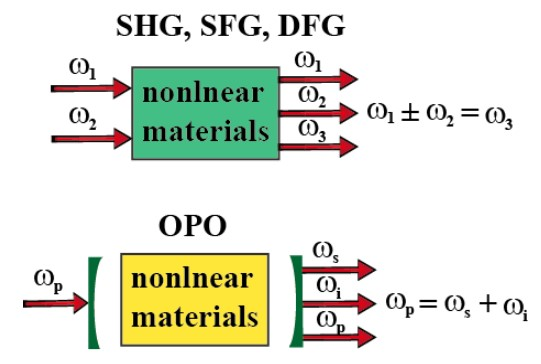
\includegraphics[width=0.9\textwidth]{./fig2.jpg}
        \caption{二阶非线性频率变换简单的原理示意图}
    \end{minipage}
\end{figure}

二阶非线性效应只有在非中心对称的介质中才会出现。在实际的应用中,非线性系数$d$比二阶极化张量$\chi^{(2)}$的使用更广泛,这两者之间的相互关系如下:

\begin{equation}
    d_{il} = \frac{1}{2}\chi^{(2)}_{ijk}
\end{equation}

由于置换对称性,两种表示方法的对应关系如下:

\begin{align}
jk:& 11 \ 22 \ 33 \ 23,32 \ 13,31 \ 12,21 \\
    l:& 1 \ 2 \ 3 \ 4 \ 5 \ 6
\end{align}

经过简化后,二阶非线性极化与输入光场电场的关系可以表达成如下形式:



\subsection{二阶非线性过程的耦合波方程描述}

光波在非线性非磁性介质中的传播可以用以下的非线性波动方程来描述:

\begin{equation}
   \nabla \times \nabla \times E + \mu_0 \sigma \frac{\partial E}{\partial t} + \frac{1}{\varepsilon_0 c^2} \frac{\partial^2 D}{\partial t^2} = -\frac{1}{\varepsilon_0 c^2} \frac{\partial^2 P^{NL}}{\partial t^2} 
\end{equation}

介质的极化率分为线性和非线性部分,即:
\begin{equation}
    P = P^{L} + P^{NL}
\end{equation}

D是线性电位移矢量,它的定义如下:

\begin{equation}
    D = \varepsilon_0 E + P^L
\end{equation}

引入一些假设:

\begin{enumerate}
    \item 假设入射光场是沿z轴传播的准单色平面波
    \item 假设在相互作用过程中,电场与极化波包振幅随距离和时间变换非常缓慢,这样它们对传播距离和时间的二阶微分可以忽略,这就是通常所谓的缓变振幅近似(Slowly-Varying Envelope Approximation, SVEA)
\end{enumerate}

最后方程可简化为:

\begin{equation}
    \frac{\partial E}{\partial z} = - \alpha E + i \frac{\mu_0c\omega}{n}P^{NL}
\end{equation}

其中,$\alpha = \frac{\mu_0\sigma c }{2}$是介质的损耗系数。

最后得到一组耦合波方程:

\begin{align}
    \frac{\partial E_1}{\partial z} &= -\alpha_1 E_1 + i \frac{\omega_1d_{eff}}{n_1c}E_3E_2^{*}e^{-(k_3-k_1-k_2)z} \\
    \frac{\partial E_2}{\partial z} &= -\alpha_2 E_2 + i \frac{\omega_2d_{eff}}{n_2c}E_3E_1^{*}e^{-(k_3-k_1-k_2)z} \\
    \frac{\partial E_3}{\partial z} &= -\alpha_3 E_3 + i \frac{\omega_3d_{eff}}{n_3c}E_1E_2e^{-(k_3-k_1-k_2)z}
\end{align}

其中$\Delta k = k_3 - k_1 -k_2$ 是三波混频过程中的位相失配,$d_{eff}$是有效非线性系数,其具体的表达式取决于入射光场的偏振和位相匹配条件

\subsection{准相位匹配技术}

准相位匹配是用来补偿非线性相互作用过程中不同频率波长光的相速差的一种技术。
在准相位匹配中,光束在传播过程中累积的位相失配可以通过周期性的改变介质的极化方向来弥补。
这样,非线性介质在光的传播方向上被周期性的改变就可以避免能量从产生的光束中转移。
在铁电晶体中,可以通过周期性改变晶体固有的电筹的方向来实现,因此相当于引入了一个有效的光栅矢量$k_Q$



\subsection{准相位匹配基本理论}

在准相位匹配晶体中,相互作用光之间的相速度失配可以用一个周期性调制的非线性系数$d$来描述,将周期性的非线性系数傅里叶展开成如下形式:

\begin{equation}
    d(z) = d_{il} \sum_{m=-\infty}^{\infty} G_m e^{i k_{mQ} z}
\end{equation}

$G_m$是m次谐波的傅里叶系数,m阶光栅矢量定义如下:

\begin{equation}
    k_{mQ} = \frac{2\pi m}{\Lambda}
\end{equation}

这里$\Lambda$是空间调制周期。第m阶空间谐波所对应的有效非线性系数为:

\begin{equation}
    d_{eff}^{(m)} = d_{il} G_m
\end{equation}

当非线性系数的符号被周期性调制,那么第m次傅里叶系数可以表达成如下形式:

\begin{equation}
    G_m = \frac{2}{m\pi} \sin{m\pi D}
\end{equation}

在这里$D$是占空比,取决于反转的电筹长度与调制周期$\Lambda$的比例。在最佳的占空比下,正弦函数取值为1,因此:

\begin{equation}
    d_{eff}^{(m)} = \frac{2}{m\pi}d_{il}
\end{equation}

\subsection{倍频中的准相位匹配}

下面以一阶准相位匹配PPKTP晶体中的倍频为例,介绍准相位匹配中的相关概念以及通常所关心的物理参数如何计算。
对于I型位相匹配,基频与倍频光的偏振方向为$E_{F}^{z}E_{F}^{z} \rightarrow E_{SHG}^{z}$。其位相失配为:

\begin{equation}
    \Delta k^{I } = k_{SHG} - 2k_{F} - \frac{2\pi}{\Lambda ^{I}}
\end{equation}

这样I型位相匹配的极化周期为:

\begin{equation}
    \Lambda^{I} = \frac{\lambda_F}{2(n_{SHG}-n_{F})}
\end{equation}

在这里,$n_F$和$n_{SHG}$为基频与倍频光在晶体$z$轴方向的折射率。

同理可得II型位相匹配的极化周期:

\begin{equation}
    \Lambda^{II} = \frac{\lambda_F}{2(n_{SHG}^y-n_{F}^y-n_{F}^z)}
\end{equation}

下图给出了不同基频光波长下I型和II型位相匹配条件下的极化周期。从图中可以看出II型位相匹配的光栅周期要大于I型位相匹配。长波长的光栅周期要大于短波长的光栅周期。

\begin{figure}[H]
    \centering
    \begin{minipage}[b]{0.9\textwidth}
        \centering
        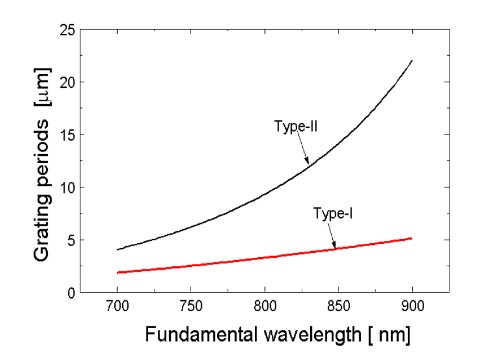
\includegraphics[width=0.9\textwidth]{./fig3.jpg}
        \caption{I型和II型匹配条件下极化周期与基频光波长之间的关系}
    \end{minipage}
\end{figure}

在倍频过程中位相匹配依赖于很多物理参数,比如温度、波长以及相互作用光束的偏振。
通常在固定其他参数,改变某一单一参数,
引起的倍频功率下降到最大功率一半时所对应参量的宽度定义为位相匹配容差,或者叫接收带宽。
对于一个有效长度为L的晶体,其位相匹配因子决定于函数$sinc^{2}(\frac{\Delta k L}{2})$。
全宽半高(Full Width at Half Maximum, FWHM)接收带宽为:

\begin{equation}
    \frac{\Delta k L}{2} = 0.4429\pi
\end{equation}

这里$\Delta k$依赖于晶体的温度以及基频光的波长。
对于I型为相匹配,在固定晶体温度时,其波长接收带宽为:

\begin{equation}
    \Delta \lambda_{FWHM} = \frac{0.4429\pi}{L}\abs{\frac{n_{SHG}-n_{F}}{\lambda_F}- \frac{\partial n_F}{\partial \lambda} - \frac{1}{2}\frac{\partial n_{SHG}}{\partial \lambda}}^{-1}
\end{equation}

当基频光的波长固定时,倍频的温度接收带宽为:

\begin{equation}
    \Delta T_{FWHM} = \frac{0.4429\pi}{L}\abs{\alpha(n_{SHG}-n_{F})- \frac{\partial n_F}{\partial T}\big{|}_{T=T_0} + \frac{\partial n_{SHG}}{\partial T}\big{|}_{T=T_0}}^{-1}
\end{equation}

公式中$\alpha$是材料的热膨胀系数,$T_0$表示某一特定的位相匹配温度。

\subsection{高斯光泵浦下的倍频功率与倍频效率的关系}

在高斯光泵浦下,在满足相位匹配的条件下,其倍频转换效率与基频光功率、晶体参数和光束聚焦参数之间的关系如下:

\begin{align}
P_{SH}=\Bigg(\frac{2\omega_{F}^{2}d_{eff}^{2}k_{F}P_{F}^{2}}{\pi n_{F}^{2}n_{SH}\varepsilon_{0}c^{3}}\Bigg)Lh(B,\zeta), \\
\zeta=L/b,\quad b=2\pi n_F\omega_0^2/\lambda_F 
\end{align}

其中, $\omega_F, k_F, P_F, n_F$ 分别为基频光的角频率、波矢、功率、折射率; $n_{S H}$ 为倍频光的折射率; $\varepsilon_0$ 为真空介电常数; $\mathrm{c}$ 为光速; $\mathrm{L}$ 为晶体长度; $\xi$ 为归一化聚焦因子; $\mathrm{b}$ 为光束在晶体中的瑞利距离 2 倍; $\mathrm{B}$ 为走离角参数; $d_{e f f}$ 为有效非线性系数。可以看出倍频输出功率是基频光输入功率的二次方关系。

倍频转换效率一般有两种定义,一种是倍频光功率与基频光功率的比值,表达式如下:

\begin{equation}
    \eta=\frac{P_{S H}}{P_F}=\left(\frac{2 \omega_F^2 d_{e f f}^2 k_F P_F}{\pi n_F^2 n_{S H} \varepsilon_0 c^3}\right) \operatorname{Lh}(B, \zeta)
\end{equation}


另一种是归一化的功率效率,对泵浦功率和晶体长度进行归一化处理,方便对比不同非线性材料的倍频性能,表达式如下:

\begin{equation}
   \eta_{\text {norm }}=\frac{P_{S H}}{P_F^2 L}=\left(\frac{2 \omega_F^2 d_{e f f}^2 k_F}{\pi n_F^2 n_{S H} \varepsilon_0 c^3}\right) h(B, \zeta) 
\end{equation}

\section{实验内容}

\begin{figure}[H]
    \centering
    \begin{minipage}[b]{0.9\textwidth}
        \centering
        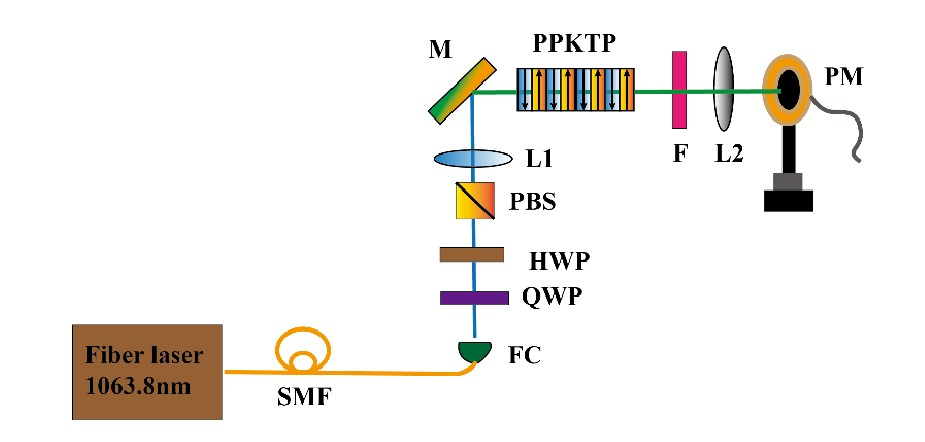
\includegraphics[width=0.9\textwidth]{./fig1.jpg}
        \caption{实验装置示意图}
    \end{minipage}
\end{figure}

实验光路图如上图所示,泵浦激光为1064nm光纤激光器,
通过光纤准直头输出到自由空间中,其偏振通过四分之一波片和半波片进行控制。
通过旋转偏振状态改变通过偏振分束器的功率大小;
过偏振分束器后,用透镜L1将泵浦1064nm激光聚焦进PPKTP晶体;
其中PPKTP晶体的温度通过半导体制冷装置精确控制;
倍频后的532nm倍频激光通过短通滤波器进行滤波再经透镜L2准直;
基频光金和倍频光的功率通过功率计进行测量。

实验流程如下:

\begin{enumerate}
    \item 打开激光器和温度控制器对仪器进行预热和准备
    \item 调节半波片和四分之一波片使得透过PBS的1064nm的光功率最大
    \item 调节晶体温度使得输出的倍频光功率最大
    \item 旋转波片,记录不同泵浦功率下的倍频激光功率
    \item 在最大泵浦功率下,调节晶体温度,记录倍频功率与温度的干涉曲线
\end{enumerate}

\end{document}